\chapter{Prototype: Implementation}
The prototype was created as previously described and was followed by two formative evaluations. One with LAER Lab and the second in the form of an on-line questionnaire after participants watched a video demo. 

\section{Game play}

\subsection*{House environment overview}
The environment consisted of two bedrooms(one empty), a kitchen and a living-room, an overview of which can be seen in \ref{old_house}. It was kept open with no doors and thus no loading required between rooms. The house architecture was designed in sketchup and imported into Blender to be tidied and imported into JMonkey. Some models (such as furniture and the character) were taken from on-line resources such as blendswap.com.  

\begin{figure}[H]
\centering
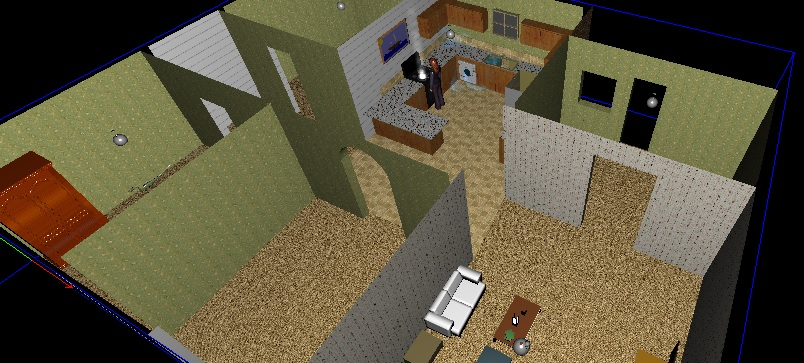
\includegraphics[width=90mm]{images/prototype/old_fullhouse.jpg}
\caption{Overview of the house used in the prototype}
\label{old_house}
\end{figure}

The living room in \ref{prototype_livingroom} contains three interact-able objects, a TV, lamp on the table as well as a ceiling light, the latter two which affect the sensory system and if not turned off or the user is too close can result in an overload. 

\begin{figure}[H]
\centering
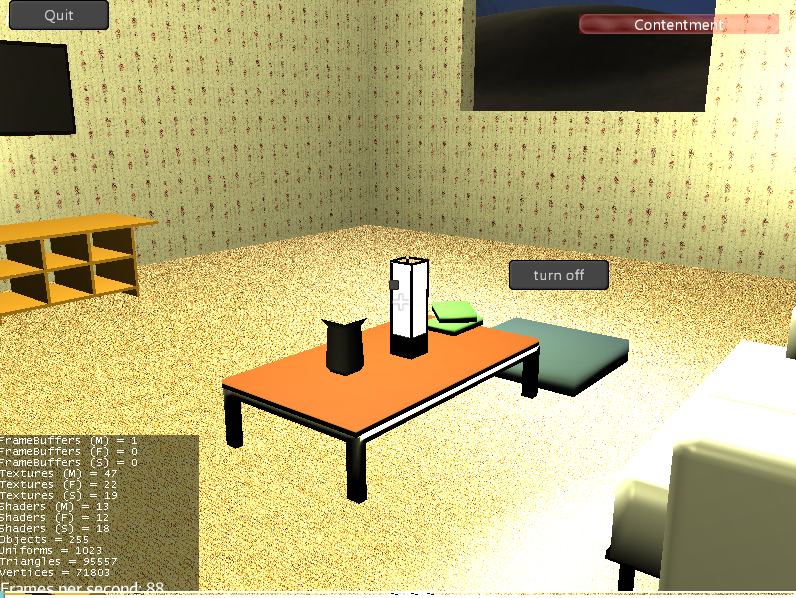
\includegraphics[width=100mm]{images/prototype/livingroom.png}
\caption{Livingroom}
\label{prototype_livingroom}
\end{figure}

The players bedroom consisted of a bed, wardrobe, ceiling light and "special interest"; a dinosaur which the user could interact with.

\begin{figure}[H]
\centering
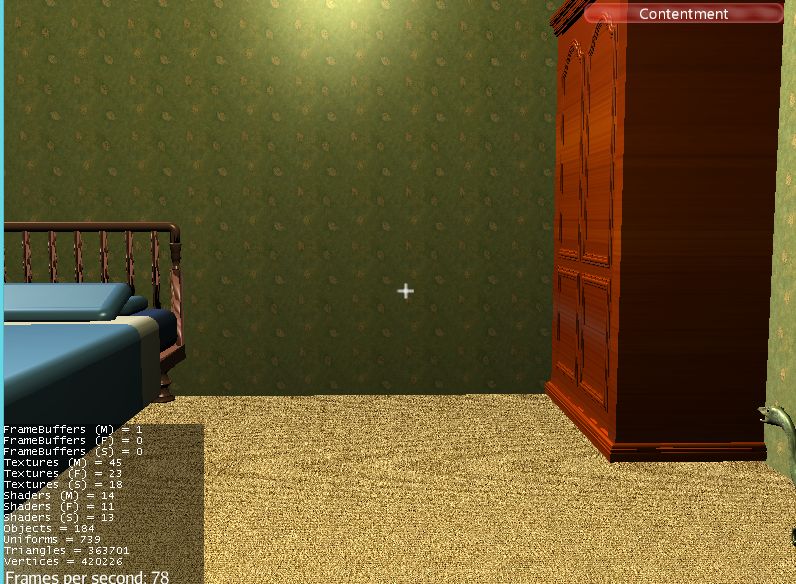
\includegraphics[width=100mm]{images/prototype/bedroom.png}
\caption{Bedroom}
\label{prototype_bedroom}
\end{figure}

The kitchen contained the parent of the game, a washing machine and ceiling light all of which were interactable. The washing machine could be turned on and off which effects the visual effects of sounds. Music notes were primarily to be used in the design, however the wanted effects could not quite be obtained and so sound waves were used instead.  

\begin{figure}[H]
\centering
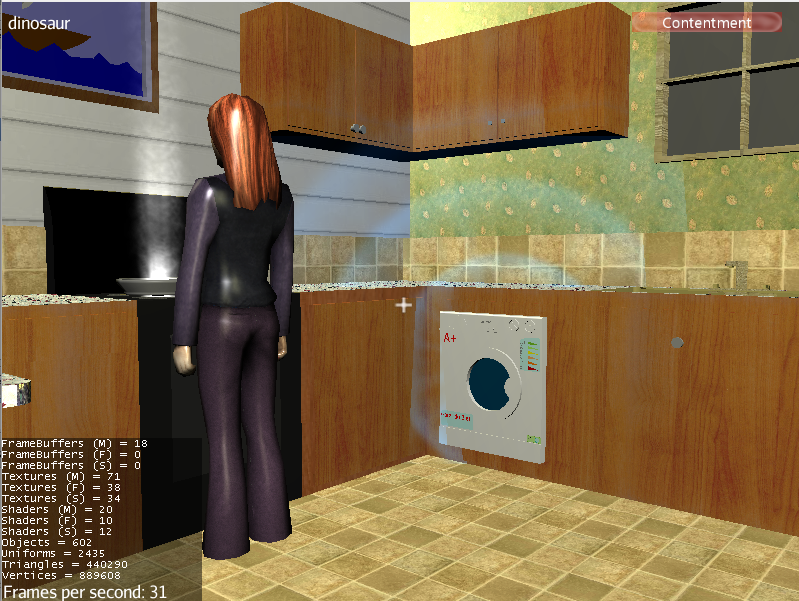
\includegraphics[width=100mm]{images/prototype/kitchen_washingm.png}
\caption{Kitchen: Visual effects from the washing machine can be seen}
\label{prototype_kitchenwash}
\end{figure}

Finally, as the game was open the user could venture outside(useful for running off if a sensory overload was occurring)

\begin{figure}[H]
\centering
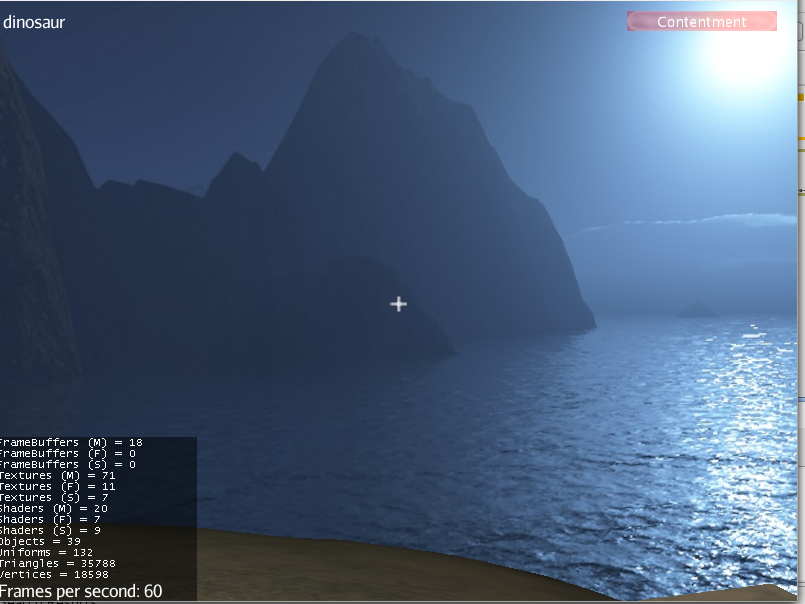
\includegraphics[width=100mm]{images/prototype/outside.png}
\caption{The peaceful outdoors!}
\label{prototype_kitchen1}
\end{figure}

\subsection*{Interactions}

The user can interact with various objects in the scene; some would provide information in the form of description boxes whereas others directly affected game play such as lights and special interests. When available actions appear for selection, the camera is disabled enabling the user to select them with their mouse as can be seen in \ref{prototype_dino}.

\begin{figure}[H]
\centering
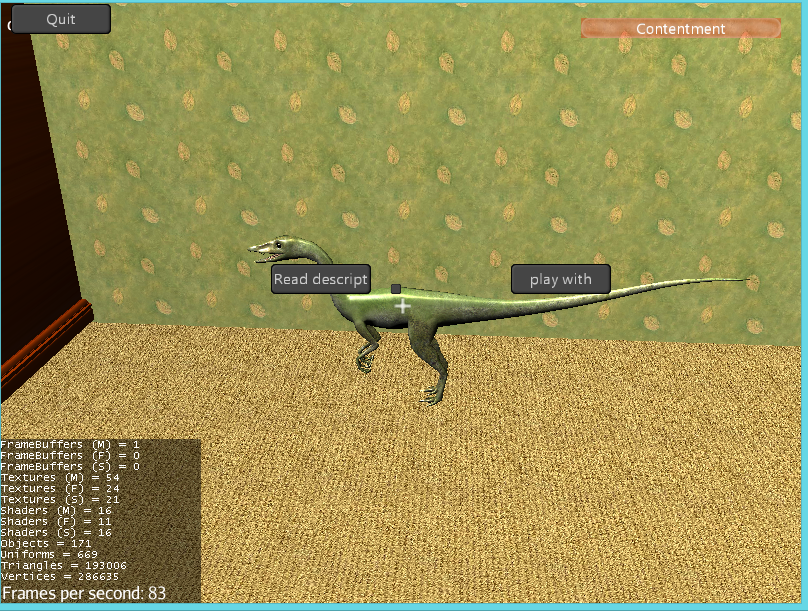
\includegraphics[width=100mm]{images/prototype/si.png}
\caption{Interacting with a special interest. Two actions available for selection can be views}
\label{prototype_dino}
\end{figure}

When the user interacts with the dinosaur(\ref{prototype_dino}), contentment increases although there was little visual indication of doing this(apart from the contentment visually increasing) and if the player was far away from the object, playing would stop. If a sensory overload was occurring and the player moved to the dinosaur quick enough they could prevent a meltdown by increasing contentment although interacting with the object would not specifically stop sensory overloads and should be implemented at a later date. 

\begin{figure}[H]
\centering
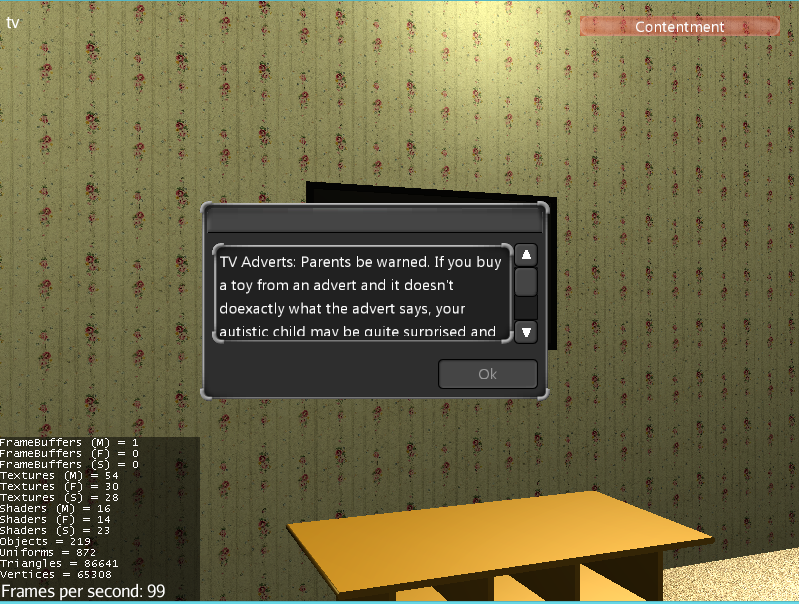
\includegraphics[width=100mm]{images/prototype/tvdescription.png}
\caption{TV description box pop-up, giving warnings of that a child may literally interpret what they see on TV }
\label{prototype_tvdesc}
\end{figure}

Only a few descriptions in the prototype were implemented. Wardrobe, frying pan, TV, dinosaur and one of the issues that arose came during sensory overloads. If one was occurring whilst reading a description the user either had to close it quickly and move away or continue to read and risk a meltdown; which if this occurs the game will reset and the user won't be able to view the description information. This is not ideal behaviour; preventing useful or important information being read.

\subsection*{Sensory overloads and meltdowns}

Sensory overloads occur when being too close to too many hazardous objects and it was was broken down into two stages, the first of which results in lights and the environment becoming brighter as can be seen in \ref{prototype_so1s1} and \ref{prototype_so2s1}. 

\begin{figure}[H]
\centering
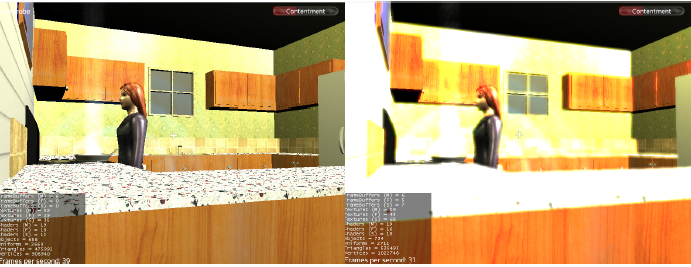
\includegraphics[width=100mm]{images/prototype/old_sensoryeffects.png}
\caption{Sensory overload effects at stage 1: The image on the left demonstrates a view with no effects. The image on the right is the result of the Bloom filter being applied resulting in lights and the environment becoming brighter}
\label{prototype_so1s1}
\end{figure}

\begin{figure}[H]
\centering
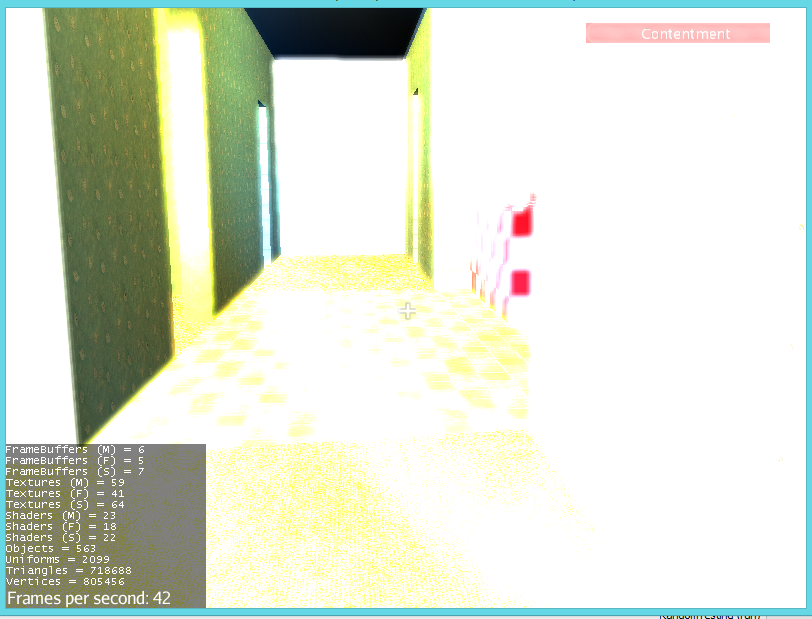
\includegraphics[width=100mm]{images/prototype/hallway_so1.png}
\caption{Sensory overload effects at stage 1: hallway extremely bright as there's lots of lighting causing issues}
\label{prototype_so2s1}
\end{figure}

If the user does not deal with this quickly enough by turning off the source of disturbance or moving away the second stage is entered which can be seen in \ref{prototype_so1s2} and \ref{prototype_so2s2}. 

\begin{figure}[H]
\centering
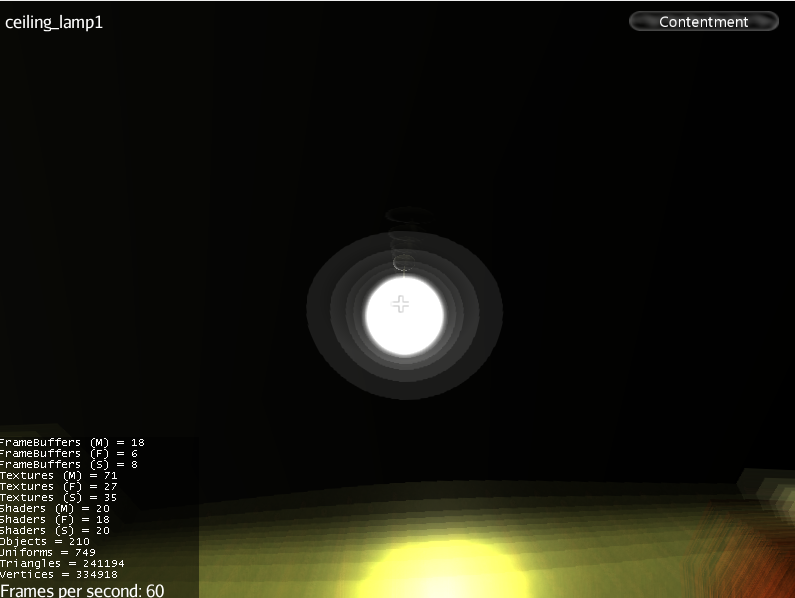
\includegraphics[width=100mm]{images/prototype/bedroom_lightsensory.png}
\caption{Sensory overload effects at stage 2: Light is much brighter and the Gaussian blur filter is applied}
\label{prototype_so1s2}
\end{figure}

\begin{figure}[H]
\centering
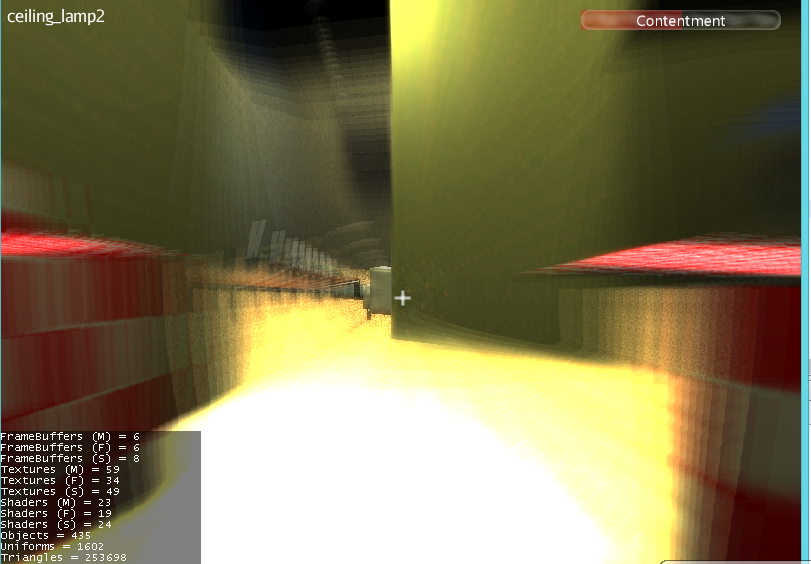
\includegraphics[width=100mm]{images/prototype/so_kitchen.png}
\caption{Sensory overload effects at stage 2: Gaussian blur filter is applied and full sensory overload is occurring}
\label{prototype_so2s2}
\end{figure}

Translating the information from interviews and readings to implementation had proved challenging because of the amount of differing information. The specific triggers do require work and adjustment, for example having only certain types lighting causing problems as currently all of them are. In addition, certain lights should only cause sensory overloads when the user is looking directly into them. Sound is currently represented by visual sound waves emitting from objects and these need to be made bigger and more dense as to cause more visual distortions.

\subsection*{Game modes}
When the simulator first starts the user can select either Explore or Mission mode with a few other options such as "About" and "Help". These cannot be switched during play and the simulator needs to be restarted to change modes. 

In mission mode, two tasks were given: to get a drink and to get dressed. When the user gets dressed, contentment drops due to tactile sensory problems; on completion(assuming the character does not have a meltdown) the next mission is selected. 

Next to the sink as in \ref{prototype_kitchenwash} is the washing machine which combined with the lighting quickly creates a sensory overload. As a representation of "Getting a drink" an action indicator(similar to a health car) is used(see \ref{prototype_actionindicator}) and when displayed the user cannot move. It slowly reduced over time and upon completion the user can move again. Thus, they are fixed at the sink until the action of getting a drink is complete, having a few seconds to run or move away before a meltdown occurs. If the contentment is too low before the task is attempted a meltdown will occur during it and in either case, the player restarts in the bedroom to attempt again. 

\begin{figure}[H]
\centering
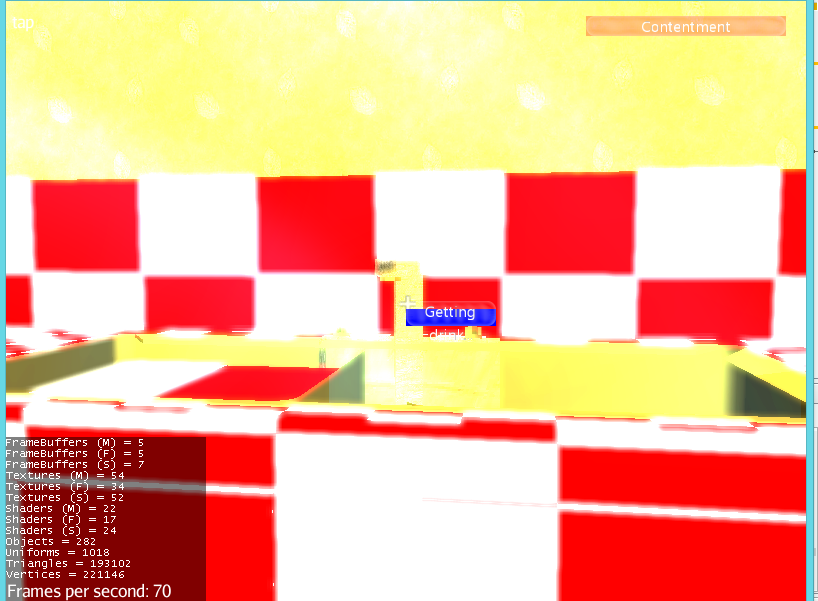
\includegraphics[width=100mm]{images/prototype/actionindicator.png}
\caption{Blue action indicator: (Texture is broken in the prototype when I tried to take this image which is why things are appearing red and white, not hard to fix but no need atm)}
\label{prototype_actionindicator}
\end{figure}

\section{Implementation: technical}

\begin{figure}[H]
\centering
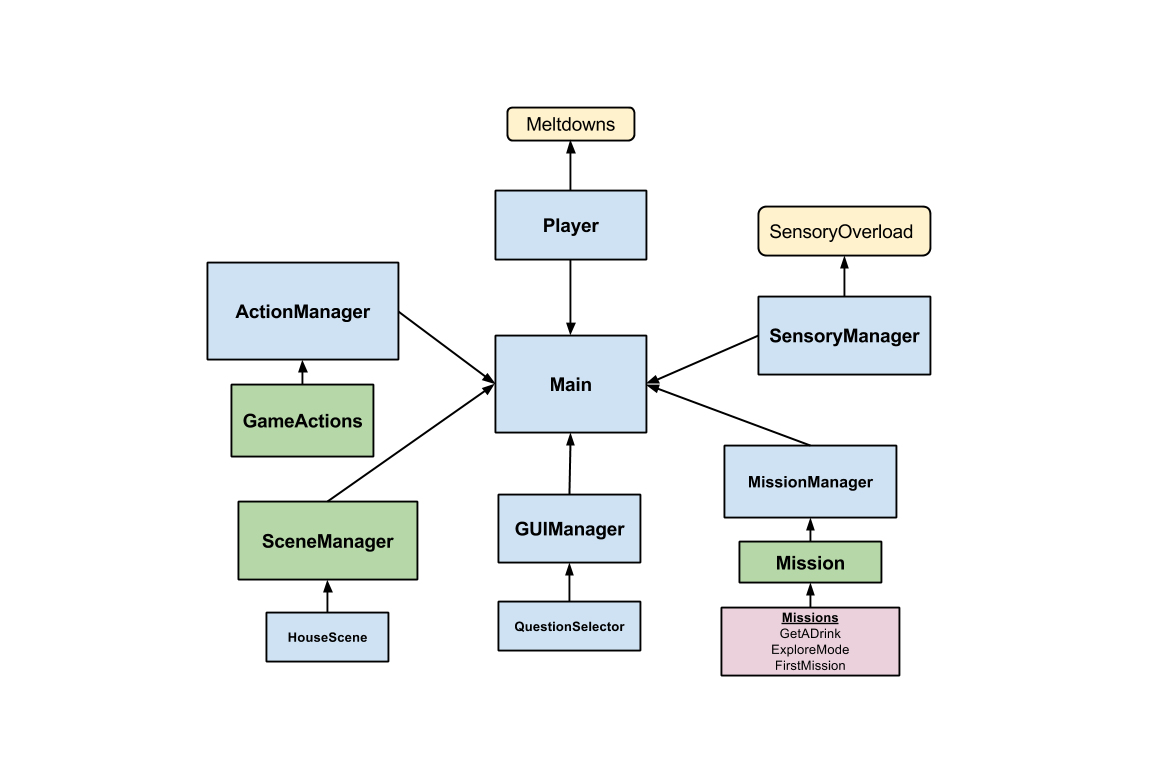
\includegraphics[scale=0.6]{images/prototype/prototypeoverview.png}
\caption{Overview of prototype design}
\label{protooverview}
\end{figure}

The prototype has several main parts:
\begin{enumerate}
\item Main: Contains the main game loop, initialises and updates all other important aspects of the simulator.
\item ActionManager: handles all the actions and interaction the player can do such as turning on and off lights.
\item GUIManager: handles all the GUI. Missions and the rest of the system can make calls to this which decides what and when to display elements. 
\item Player: Represents the player and state of the player in the game(such as current contentment level). Contains methods for internal actions such as "getDressed", calculates reduction in contentment which is dependent on the current state of the player(if not interacting with a special interest or experiencing a sensory overload) and contains methods for starting and stopping meltdowns.
\item SensoryManager
\item SceneManager: Anything that represents a scene extends this and inherits useful methods for setting up a scene. In our case this is a house. 
\end{enumerate}

Terminology used in JMonkey
\begin{enumerate}
\item Spatial: Spatials represent nodes or a geometry in a scene, from a teapot to the root node which contains the entire scene. All models created by blender are converted into spatials. Spatials can be searched and children can be added.
\item Controls: controls are game logic components which are added to control spatials. For example, a movement control could be added to a dog spatial which would repeatedly make it walk around. Multiple controls can be added to spatials making it a very modular feature that JMonkey offers. 
\item AbstractState: can be used to control game logic and are only active once they are attached to JMonkeys state manager.
\end{enumerate}

\subsection{SceneManager}
In JMonkey, scenes are created by adding spatials to a scene file which has the extension of .j3o. All models created in blender area converted to .j3o files and can be translated and rotated in order to create the scene by using JMonkeys inbuilt scene graph. The scenes are loaded into the asset manager which can be accessed by the scene that is loaded which in our case is the HouseScene. A new scene is created by specifying the Scene.j3o spatial name and upon initialisation it would load all the spatials(models) into a hashmap <String, Spatial> so that the rest of the system had quick access to spatials by their key(name of the object) and would thus not have to constantly search the scene graph to find objects of interest which could later be an optimisation issue. 

"SceneManager" is an abstract class so new scenes could be easily created and could use methods that would be commonly required and could setup requirements such as:

\begin{enumerate}
\item Descriptions to objects such as the fryingpan, wardrobe and tv which would appear as description boxes. 
\item The player starting point and respawn point after a meltdown must be set by the scene. 
\item Sensory object types and adding these to the sensory manager for computation when the scene was loaded. 
\item Setup custom materials that may be used in the scene
\end{enumerate}

The SceneManager contained methods such that common sensory objects were created on initialisation based on the name of the spatials rather than needing to constantly use addSensoryObject methods. The SceneManager would go through all the objects in the scene and found ones that had the name "lamp" and would then assign this as a light sensory object and add point lights saving a lot of work for the developer creating new scenes and scenarios. Pointlights had to be added to root node the the scene in order to make sure lights affect all models around it otherwise it would only influence the node it was attached to, for example if attached to a lamp only the lamp would be lit and not the surrounding objects. The better alternative to adding point lights would be to create materials in blender to represent the lighting however this was a lot of modelling work; the problem with pointlights is that it doubles the amount of vertices in the scene for each one added.

\subsection{GUIManager}
At the time the prototype was developed a new GUI package became available for JMonkey. Although it is still in beta with little documentation it provided a faster method of creating the GUI and and required components. 

The main game loop calls the update method in the GUIManager. The GUIManager controls, adds and updates virtually all of the interface and elements such as the contentment indicator, action indicator, displaying of description boxes and action selection, storing any selected actions for Main to request. 

The most important aspect of the GUIManager is the control of the "QuestionSelector", a component made for users to select actions or respond to questions from other in-game characters. The QuestionSelector takes three pieces of information: questions, answers and a boolean to indicate whether or not actions should be rotated and is additionally used to represent information processing delay.


\subsection{ActionManager}
The ActionManager can be broken down into the most important methods:

\begin{enumerate}
\item getActions(Spatial): gets the available actions the user can use on the spatial.
\item doAction(GameActionEvent gae): fires a GameActionEvent which simply contains the name of the action and the spatial to act upon.
\item notifyGameActionListeners: notifies all listeners of an action event
\item getType(Spatial s): gets the type of a spatial which defines which actions can be used on it although custom types can be added. These mostly would depend on the name of the spatial, for example anything that contained the name "lamp" would be assigned the "lamp" type however custom types from missions or scenes could be added so that actions only needed for certain missions such as "get a drink" would only be available during the mission.
\end{enumerate}

If the user clicks on a spatial, using collision detection it is calculated which spatial they have clicked on. It would then use getActions(Spatial s) to acquire which actions the spatial has, based on it's type, and send this to the GUI to display the question selection.

Once the user selects an action the GUI fires doAction which decides what to do about it.

\subsubsection*{Types implemented}
*** put this in a table I think and  cleanup with above, doesnl't need a whole section.

If the spatial is of type "lamp", it would call changeLight(spatial) which is in GameActions and the spatial is searched for an associated point light to change depending on it's current state. 

If the spatial was type "sound", a particle emitter would be added or removed from the spatial depending on it’s current state(if its on or off).

If the object was type "play", the action manager would call player.doAction(name). All internal player actions were in the player class, for example stim, getDressed, meltdown, pickup item, eat etc. There was other types for interacting with objects such as doors, but doors were never used in the prototype.

\subsubsection*{Custom actions and action listeners}
Custom actions can be added from missions or from scenes by implementing the GameActionListener which requires implementation of two methods, notify and getCustomGameActions. Below is an example taken from the "FirstMission"

\begin{lstlisting}
    public ArrayList<GameActionEvent> getCustomGameActions() {
        ArrayList<GameActionEvent> actionEvents = new ArrayList<GameActionEvent>();
        actionEvents.add(new GameActionEvent("Speak to", getSpatial("mum")));
        return actionEvents;
    }
\end{lstlisting}

\begin{lstlisting}
    public boolean notifyAction(GameActionEvent gae) {
        if(gae.getName().contains("Speak to")) {
            isComplete = true;
            return true;
        }
        return false;
    }
\end{lstlisting}

This approach was used to provide modularity so that actions and gameplay in missions was not restricted by the system(a developer could create their own actions and interactions) however still ensuring some level of implementation a developer would not have to implement. I.e lights, sounds, etc.

Once the listener is added to the action manager it will call getCustomActionEventsTypes() which would return all the custom actions added from either scenes or missions and allow the user to select a custom action. doAction would then attempt the action which if it was custom would not be found. At the end of every doAction it notifies all gameaction listeners. Thus missions can listen on to what the user is doing and act accordingly. 


\subsection{Player}
The player class contained the players location and general states such as if objects were being held, if we are interacting with a special interest or in a state of a meltdown.

The main update loop of the player is called from the Main class and it constantly checks the state of the sensory manager which could be NONE, MEDIUM, OVERLOAD. Depending on this state the class will use filters to create the sense of a sensory overload or when the user is nearing one whilst reducing contentment accordingly. If in MED a light filter is applied to make lights get brighter and if in a sense of overload both the light filter and guassian filter are applied. The player update loop can be seen in the appendix.  
 
\subsubsection{Meltdowns}
When contentment dropped below 15 a meltdown would start and progressively get worse which would give the player a few seconds to attempt to prevent it. When a meltdown starts the first person camera starts to shake giving warning; and then gets progressively worse to the point the game is not playable. 

Meltdown events were fired after meltdown had occurred and been stopped. Anything that implemented the meltdown listener would be notified. This was so missions could handle meltdowns if wanted to be done in a different way instead of simply forcing the player to restart at a respawn point. It also meant that missions could give custom messages and prompt users or give hints if meltdowns were occurring too frequently.


\subsection{Sensory Manager}

Sensory objects setup in the scene and are added to the sensory manager in an arraylist. The manager looks through the arraylist and compares distance from player to these objects. If the distance is below a set threshold it is deemed within proximity to the player and is included in the sensory overload calculation, known as "Sensory points". Sensory points is a running total of how many objects are affecting the player and is deducted from $sensory health$. The state of the sensory manager would depend on this health and it would be set as NONE, MED or OVERLOAD. When the user came away from any sensory objects this health would slowly refill and effects would slowly subsidise. The type of object being set and only sound and light objects were initially implemented as there were no models to create a tactile sensory object and it wasn't deemed necessary at this point. 

\subsubsection{Sensory overload algorithm}
- need to do psydocode for this, better explaining than words which is complicated. 


\subsection{MissionManager}
The mission manager keeps track the current mission played, missions completed and all subsequent missions. Once a mission has been complete it will select the next one in the ArrayList. 


\subsubsection*{Missions}
Missions are AbstractAppStates and once loaded by the missions manager has defined game logic that comes into effect but only fur the duration of a specific mission. 

"Missions" extend "Mission" which is an abstract class and contains methods that mission states may frequently need with a goal for development of to be as simplistic as possible with no knowledge of the rest of the system required.

Missions must implement three methods:
\begin{enumerate}
\item isComplete: Mission manager will repeatedly check this and when true the mission will be detached and replaced with the next one. 
\item getMissionDescription: returns description of the mission which is displayed in the description box once loaded by the mission manager. 
\item getMissionName: return the name of the mission and is only used on initialisation. 
\end{enumerate}

In addition missions can define custom actions on objects which may only be applicable when the mission is active, e.g, get a drink, get dressed, ask Mum for help by implementing the GameActionListener. Task classes set the conditions for completion such as player the player must be holding a drink or be dressed and on completion the next task is selected and displayed to the user. One of the benefits of missions and tasks comes with testing; specific tasks can be selected and tested and it thus does not require playing an entire story to get to the parts that are required.

\section{Overcoming challenges}

// hmm, maybe move this to a discussion section? Pretty sure there's more I can yap on about here. 

At the start of the project significant amounts of time were spent trying to import rather than create models. It was a tedious task because small changes to the models required the whole house scene to be remade in JMonkey or
time had to be spent on editing models better work with JMonkeys import system. It also became evident from using Blender that it has a very steep learning curve and is a tool which can take some considerable time to master.
However, in the last two months of the game development process, these obstacles have been largely overcome. Experience acquired, coupled with updates in February to the JMonkey import system, made it easier and less
time consuming to acquire, create, change and import models. The whole scene was no longer required to be rebuilt allowing time to be better spent. Moreover, the update allowed direct use of google sketchup, a 3D modelling
tool which is easier and quicker to use than Blender (although it produces less quality assets) and offers a wealth of free models in the online repository, most of which are home components such as furniture.

Overall, JMonkey has proven to be a good choice. No additional limitations have been found and development was quick once a solution was found to the model import pipeline. The modularity offered by Java allows
further extensions to be created with ease without needing to change a large portion of the program structure. Finally, being able to combine sketchup and Blender has been a great help and with practice, asset creation should
continue to speed up.